% ============================ 四、探索过程与研究信号 ============================
\section{探索过程与研究信号}
\label{sec:signals}

\subsection{验证协议：三条不可协商项}
\label{sec:protocol}

\begin{enumerate}
\item \textbf{所有参照统计量仅在训练行上冻结}——归一化偏移、PCA 载荷、残差基线 $\bm{\mu}_{\text{ctx}}/\bm{\mu}_{\text{drug}}$、目标编码、蛋白簇索引、三维药效团 PCA、ITPV 的 SVD 基。残差基线额外带\textbf{置空保护}：把所有评测行置空后重新拟合，结果必须逐位相同。这与修订后手册第 2.2 节第 15 条的补充口径完全一致：\emph{验证集与测试集均不得参与训练，也不得用于估计任何统计量（含保留蛋白列表与归一化参数）}。
\item \textbf{官方划分边界不被改动}——\code{split\_final} 字段冻结给出的 train/val 边界原样使用；我们仅在 \code{train} 划分\emph{内部}做五折留化学组交叉拟合用于模型选择，这也正是修订后手册第 2.2 节第 6 条允许的做法。
\item \textbf{验证集只被评分一次}，且\textbf{目标预注册}——每阶段的成功判据在实施前写入计划文件。
\end{enumerate}

\begin{table}[H]
\centering\small
\caption{\textbf{预注册目标与实际结果。} 两次未达成均按原样报告并用于诊断，未被回溯改写为重新定义的目标。}
\label{tab:targets}
\begin{tabular}{clcc}
\toprule
阶段 & 预注册目标 & 实际结果 & 判定 \\
\midrule
2 & 复现按官方分组实现的均值基线 & 0.445443（逐位复现） & 达成 \\
3 & 验证总分 $>0.4454$（超越基线） & 0.436172 & \textbf{未达成} \\
4 & 验证总分 $>0.4550$ & 0.477377 & 达成 \\
5 & 验证总分 $>0.4900$ & 0.508552 & 达成 \\
6 & 验证总分 $>0.5150$ & 0.508655 & \textbf{未达成} \\
6 & ITPV 通过事先声明的药理学对照 & 阳性 11/12、阴性 10/10 & 达成 \\
\bottomrule
\end{tabular}
\end{table}

\subsection{六阶段轨迹与两个队列的成绩}

\begin{table}[H]
\centering\small
\caption{\textbf{六阶段成绩轨迹（两个队列）。} 验证列由离线口径在验证队列（2\,806 例受扰样本 $\times$ 5\,243 蛋白）上计算，协议为\textbf{权重冻结于折外队列、验证集仅评分一次}；\NEW{}测试列为依据修订释放的真值在测试队列（4\,226 例）上的\emph{自评}，\textbf{非官方分数}。第 3、6 阶段均未达到其预注册目标，按原样记录。}
\label{tab:headline}
\begin{adjustbox}{max width=\textwidth}
\begin{tabular}{clcccc}
\toprule
阶段 & 主要方法 & 验证总分 & 相对基线 & 测试自评 & 相对基线 \\
\midrule
1 & 数据质控、对照匹配与 $\bm{\Delta}$ 矩阵构建 & --- & --- & --- & --- \\
2 & 评分 harness 与分布外划分（按官方分组实现的均值基线） & 0.445443 & 基准 & 0.424883 & 基准 \\
3 & 表格梯度提升（37 特征、按情形路由） & 0.436172 & $-0.009271$ & 0.393083 & $-0.031801$ \\
4 & RDKit 分子化学 $+$ 深度多任务 $+$ 折外 stacking & 0.477377 & $+0.031934$ & 0.441012 & $+0.016129$ \\
5 & 知识图谱 $+$ 五折留化学组交叉拟合 $+$ 蛋白簇 stacking & 0.508552 & $+0.063109$ & 0.463047 & $+0.038163$ \\
6 & 机制先验 $+$ 动态交叉注意力 $+$ 分层收缩 & \textbf{0.508655} & $\bm{+0.063212}$ & \textbf{0.463638} & $\bm{+0.038755}$ \\
\bottomrule
\end{tabular}
\end{adjustbox}
\end{table}

\begin{keybox}[title=核心结论（六条）]
\small
\begin{enumerate}
\item \textbf{验证总分 0.508655，较上述均值基线 $+14.2\,\%$}；测试集预测矩阵 $4\,226\times5\,243$ 通过全部 7 项致命完整性门控。
\item \NEW{}\textbf{同一结论在测试队列上同向成立}：自评总分 0.463638、同口径基线 0.424883（$+9.1\,\%$）；四个阶段相对基线的\emph{符号与次序}在两个队列上完全一致，且四种聚合口径下的差值全部为正。
\item \textbf{增益是可归因的}：交叉拟合把权重校准队列由 2\,700 行扩到 5\,078 行，单独贡献 $+0.0225$；蛋白簇权重扩展再贡献 $+0.0086$（配对自助法 1\,000 次重采样，95\,\% CI $[+0.00651,+0.00701]$，1\,000 次重复全部支持）。
\item \textbf{知识注入被独立验证为正确，却未带来预测增益}：靶点效力向量阳性对照召回 11/12、阴性对照 10/10 全零，作为特征加入后验证总分仅变动 $+0.000103$。
\item \textbf{注意力调制坍缩}：8 个化学模式的有效参与比仅 1.28，混合熵 1.215（均匀情形为 2.079）——架构的表达能力远未被数据激活。
\item \textbf{预注册目标未达成时按原样报告}：阶段 3 目标 $>\!0.4454$（实得 0.436172）、阶段 6 目标 $>\!0.5150$（实得 0.508655），两者都写在结论而非限制章节。
\end{enumerate}
\end{keybox}

\begin{figure}[H]
\centering
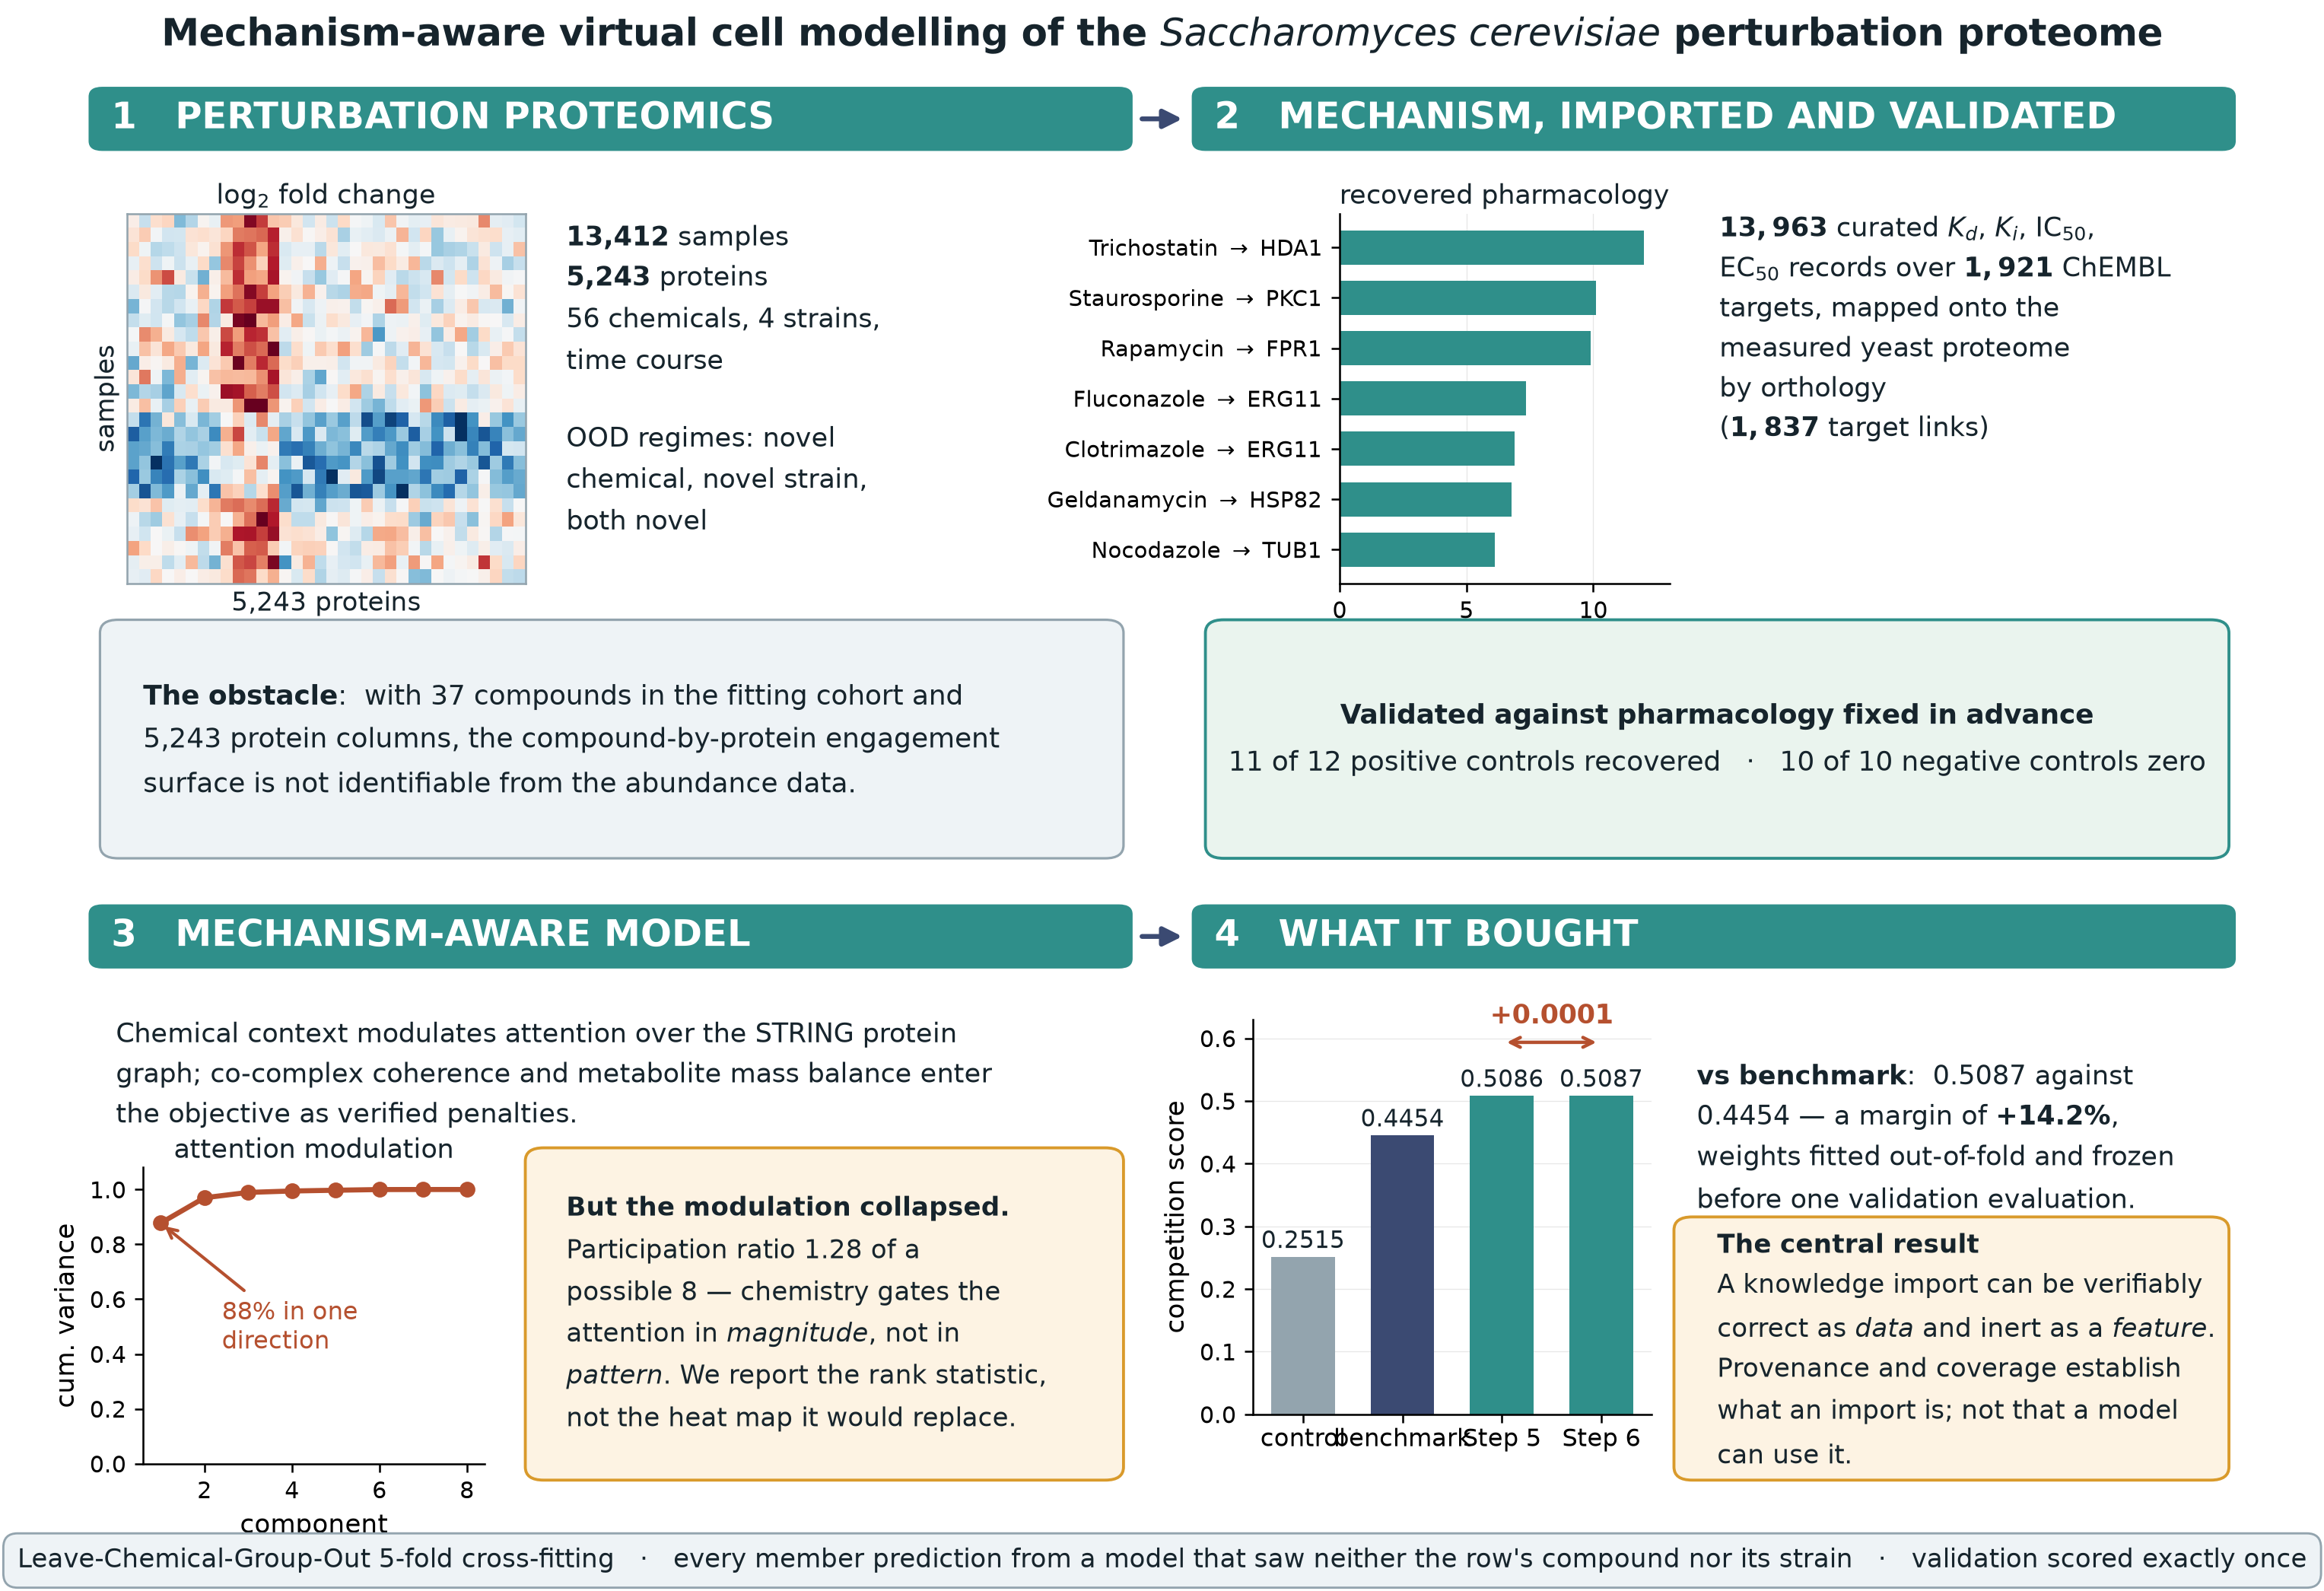
\includegraphics[width=\textwidth]{figures/step6_graphical_abstract.png}
\caption{\textbf{机制感知建模的结果总览（全部数值由结果产物在绘图时读入）。} 涵盖数据规模与质控、三源先验规模与验证、模型结构计数、六阶段分数轨迹与七模块分解。}
\label{fig:ga6}
\end{figure}

\begin{figure}[H]
\centering
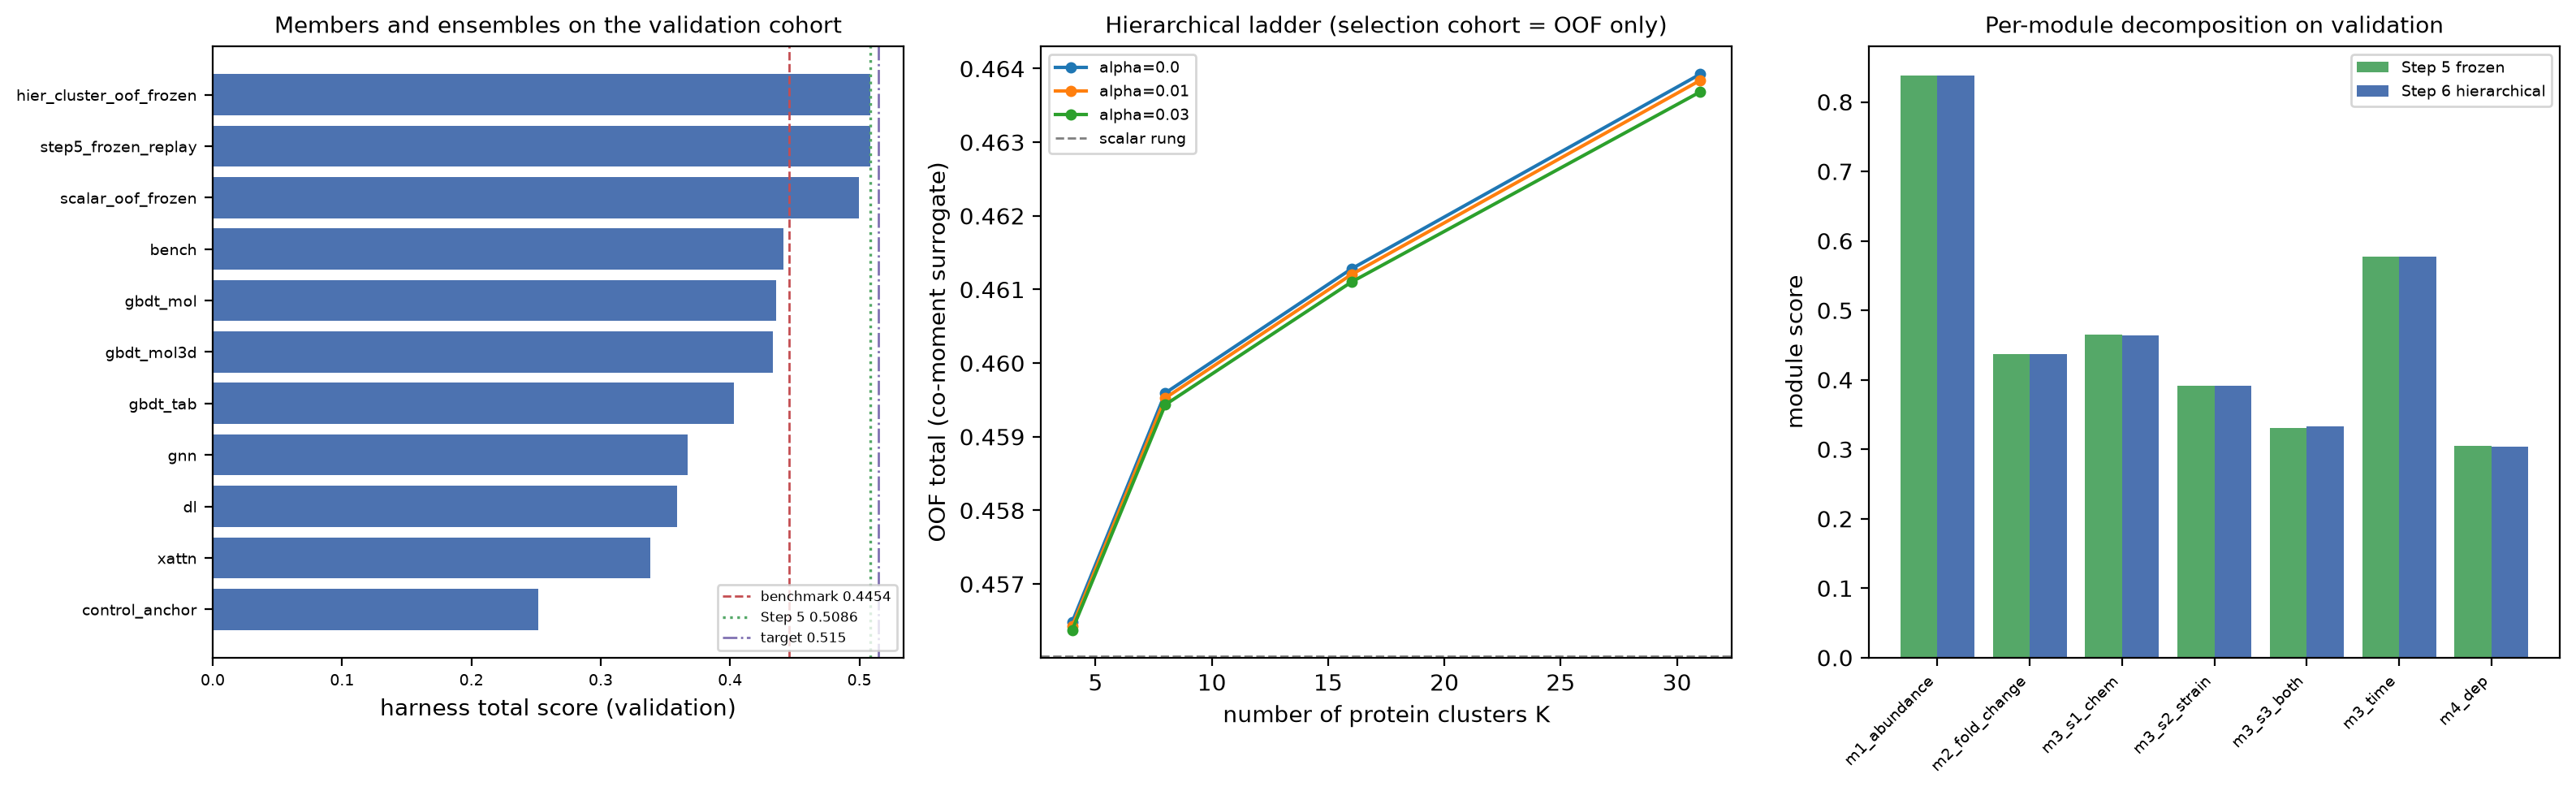
\includegraphics[width=0.97\textwidth]{figures/step6_performance_comparison.png}
\caption{\textbf{最终阶段的三项对比（验证队列）。} 左：各成员与两个集成的加权总分——注意\emph{单个神经成员（GNN 0.3674、交叉注意力 0.3381、多任务 0.3589）弱于表格成员（分子成员 0.4356）}，其价值体现在堆叠中的互补性而非单模型强度。中：分层收缩阶梯（\textbf{选择队列仅为折外队列，验证集未参与任何选择}）。右：验证集上的七模块分解。阶段 6 相对阶段 5 的分模块差异均在 $\pm0.0021$ 以内（最大者为 S3 的 $+0.0021$），总分变动 $+0.000103$。}
\label{fig:perf}
\end{figure}

\begin{table}[H]
\centering\small
\caption{\textbf{增益来源的分解与统计显著性。} 消融阶梯的两项贡献在同一队列上分离；配对非参数自助法 1\,000 次重采样（重采样单位为验证样本）。需声明区间的\textbf{作用域}：自助法只覆盖逐样本均值型子度量，占总权重 0.5875，因此是对总分差异的部分而非全部刻画。}
\label{tab:boot}
\begin{tabular}{lccc}
\toprule
比较 & 点估计差值 & 95\,\% 置信区间 & 支持比例 \\
\midrule
阶段 5 簇级 $-$ 标量（同队列） & $+0.006755$ & $[+0.006512,\,+0.007006]$ & 100.0\,\% \\
阶段 5 簇级 $-$ 基线成员 & $+0.039859$ & $[+0.037840,\,+0.041796]$ & 100.0\,\% \\
阶段 6 分层 $-$ 标量（同队列） & $+0.007146$ & $[+0.006847,\,+0.007435]$ & 100.0\,\% \\
阶段 6 分层 $-$ 阶段 5 冻结重放 & $+0.000429$ & $[+0.000282,\,+0.000586]$ & 100.0\,\% \\
\midrule
\multicolumn{4}{@{}l}{\emph{消融阶梯（同队列分离）：} 交叉拟合单独贡献 $+0.0225$；蛋白簇权重扩展单独贡献 $+0.0086$。} \\
\bottomrule
\end{tabular}
\end{table}

表 \ref{tab:boot} 的最后一行值得单独说明：阶段 6 相对阶段 5 的差异虽然区间完全位于正侧且 1\,000 次重复一致，但\textbf{点估计只有 $+0.000429$}（总分口径 $+0.000103$）。\emph{一个统计上稳定的效应仍然可以在实践上无关紧要}——本文按这两个维度分别陈述。测试队列给出的独立读数与此吻合：阶段 6 相对阶段 5 为 $+0.000592$，同样是「方向一致、幅度可忽略」。

\subsection{三项负结果与失败分析}
\label{sec:negative}

\begin{warnbox}[title=负结果一：可验证的知识导入没有带来预测增益]
\small
靶点效力向量通过了我们能设计的每一项验证（阳性 11/12、阴性 10/10、密度与覆盖度可核、SVD 解释方差 99.44\,\%），作为特征却几乎是惰性的（验证总分 $+0.000103$）。我们给出四种候选解释，并\textbf{明确指出哪一个成立尚未被实验区分}：（一）与分子结构特征\textbf{冗余}——ECFP4 与描述子可能已隐含编码靶点类别；（二）\textbf{化合物级对比不足}——37 个训练化合物无法支撑对 419 个被注释蛋白的差异化利用；（三）\textbf{评分口径不敏感}——总分由逐样本相关主导，而机制效应体现在少数蛋白上；（四）\textbf{集成已饱和}。区分它们所需的实验（逐化合物留一、机制特异蛋白子集上的分模块评分、与结构特征的正交化）\textbf{均未执行}，因此我们不主张任何一种解释。
\end{warnbox}

\begin{figure}[H]
\centering
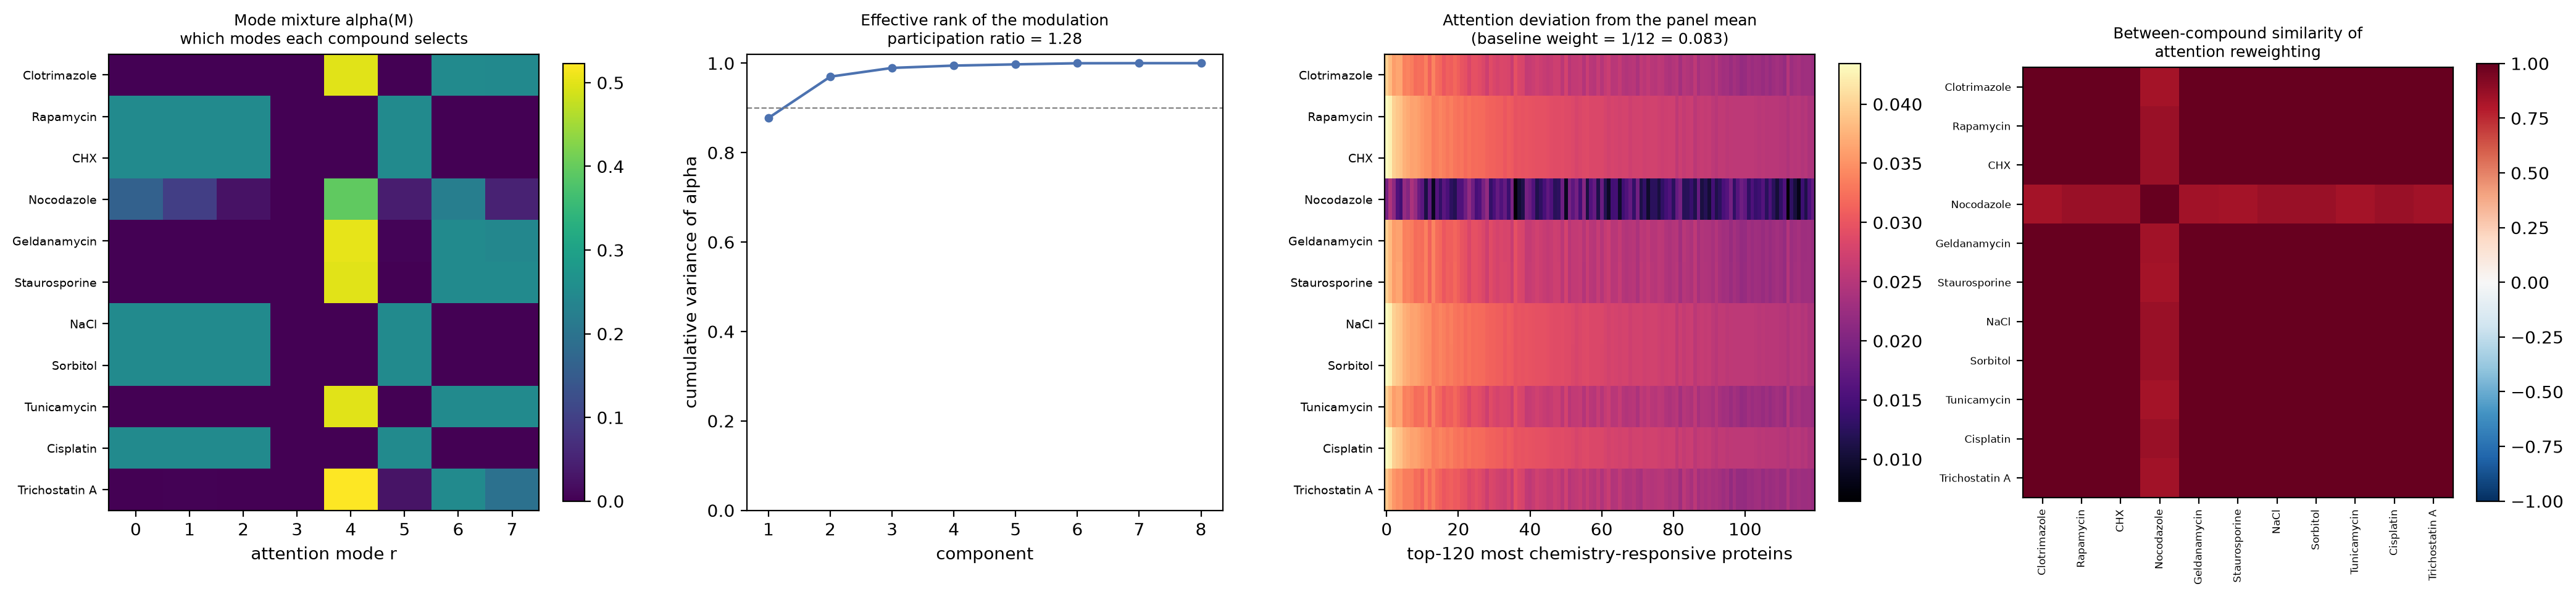
\includegraphics[width=0.90\textwidth]{figures/step6_cross_attention_weights.png}
\caption{\textbf{负结果二：交叉注意力调制坍缩。} 8 个化学模式在 43 个化合物上的有效\textbf{参与比仅 1.28}（混合熵 1.215，均匀情形 2.079；化合物间 $\alpha$ 标准差 0.103；注意力相对面板均值的最大偏离仅 0.0434，而基线注意力权重为 $1/12=0.0833$）——架构的表达能力远未被数据激活。这里有一条方法学教训值得单独记录：\textbf{同一个检查点完全可以支撑一张看起来极具说服力的非均匀注意力热图——只要不计算参与比}。定量的秩诊断与定性的可视化在此给出相反印象，说明架构「是否被激活」必须用谱量而非用图像判定\citep{jain2019attention,wiegreffe2019attention,serrano2019attention}。}
\label{fig:attn}
\end{figure}

\begin{warnbox}[title=负结果三：算力扩展的效应真实但很小，且单折会给出错误符号,breakable=false]
\small
训练轮数由 150 增至 300，五折平均开发 PCC 由 0.19545 提升到 0.20625，增益 $+0.0108$（标准差 0.0084），\textbf{4/5 折改善}，代价 0.547 GPU-小时，边际回报约 $+0.0986$ dev-PCC/GPU-小时。
这里有一个\textbf{我们自己犯过并纠正了两次}的错误：最初的比较用「中途检查点」对「整个运行的最优分数」，引入了早停选择优势；改为「终止轮对检查点」的正确定义后，增益由 $+0.0120$（5/5 折）变为 $+0.0108$（4/5 折）。此外，在只有第 0 折完成时写下的草稿曾得出「额外算力无用」的结论——\emph{而第 0 折恰恰是唯一没有改善的折}。
\textbf{结论：把轮数再翻倍是成本线性、收益未知的操作}；本方案因此不把算力扩展列为主要路线，而列为扩展项。
\end{warnbox}

\textbf{一次静默的数据库失败。} ChEMBL 结构查询曾返回有效标识符，但这些标识符指向\emph{不携带生物活性数据}的结构重复记录，使机制覆盖率减半\textbf{且不报错}。修正方式是强制解析到规范母体分子。这类失败的危险在于它不抛异常，只能靠覆盖率的绝对量级是否符合预期来发现——这也是我们坚持在每个先验上报告「实测计数」而非「已接入」的原因。

\subsection{提交完整性验证}

测试集导出经 8 项检查（7 项致命、1 项诊断）全部通过。修订后手册第 2.2 节第 16 条补充了两条格式要求——\textbf{仅接受 log$_2$ 尺度}、\textbf{蛋白列须与官方 feature contract 完全一致}——我们的门控本就覆盖这两条：预测矩阵为 log$_2$ 尺度的绝对丰度（区间 $[10.22,\,33.10]$，落在训练观测区间 $[10.16,\,33.45]$ 之内），CSV 表头为 5\,244 列（1 个 \code{sample\_ID} $+$ 5\,243 个蛋白，顺序与官方一致）。

\begin{table}[H]
\centering\small
\caption{\textbf{提交完整性门控。} 致命项失败即中止；诊断项失败只记录。这一「致命/诊断分离」的设计本身来自一次教训——阶段 4 引入的过严动态范围门在阶段 5 中止了导出，而过严的包含性门控会\emph{拒绝任何标定良好的模型、奖励一个裁剪自身输出的模型}。}
\label{tab:gates}
\begin{tabular}{@{}p{8.8cm}cp{4.6cm}@{}}
\toprule
检查 & 类型 & 结果 \\
\midrule
测试样本 ID 恰好覆盖一次 & 致命 & 通过（4\,226 / 4\,226 唯一） \\
预测矩阵蛋白维度完整 & 致命 & 通过（$4\,226\times5\,243$） \\
丰度矩阵无非有限值 & 致命 & 通过（0 个） \\
倍数变化矩阵无非有限值 & 致命 & 通过（0 个） \\
预测丰度落在训练观测区间内 & 诊断 & 满足（超出 0.00） \\
预测丰度落在放宽 2 log$_2$ 的区间内 & 致命 & 通过 \\
CSV 以预期表头解析（log$_2$ 尺度、列序一致） & 致命 & 通过（5\,244 列） \\
CSV 与 parquet 镜像一致 & 致命 & 通过 \\
\bottomrule
\end{tabular}
\end{table}
